%%%%%%%%%%%%%%%%%%%%%%%%%%%%%%%%%%%%%%%%%%%%%%%%%%%%%%%%%%%%%%%%%%%%%
%% This is a (brief) model paper using the achemso class
%% The document class accepts keyval options, which should include
%% the target journal and optionally the manuscript type. 
%%%%%%%%%%%%%%%%%%%%%%%%%%%%%%%%%%%%%%%%%%%%%%%%%%%%%%%%%%%%%%%%%%%%%
\documentclass[journal=jacsat,manuscript=article]{achemso}
\usepackage{graphicx}

%%%%%%%%%%%%%%%%%%%%%%%%%%%%%%%%%%%%%%%%%%%%%%%%%%%%%%%%%%%%%%%%%%%%%
%% Place any additional packages needed here.  Only include packages
%% which are essential, to avoid problems later. Do NOT use any
%% packages which require e-TeX (for example etoolbox): the e-TeX
%% extensions are not currently available on the ACS conversion
%% servers.
%%%%%%%%%%%%%%%%%%%%%%%%%%%%%%%%%%%%%%%%%%%%%%%%%%%%%%%%%%%%%%%%%%%%%
\usepackage[version=3]{mhchem} % Formula subscripts using \ce{}
\usepackage[breaklinks]{hyperref}

%%%%%%%%%%%%%%%%%%%%%%%%%%%%%%%%%%%%%%%%%%%%%%%%%%%%%%%%%%%%%%%%%%%%%
%% If issues arise when submitting your manuscript, you may want to
%% un-comment the next line.  This provides information on the
%% version of every file you have used.
%%%%%%%%%%%%%%%%%%%%%%%%%%%%%%%%%%%%%%%%%%%%%%%%%%%%%%%%%%%%%%%%%%%%%
\newcommand*\mycommand[1]{\texttt{\emph{#1}}}
\newcommand{\uM}{$\mu$M }

\author{William McCorkindale}
% \affiliation{Cavendish Laboratory, University of Cambridge, Cambridge CB3 0HE, United Kingdom}
% \altaffiliation{A shared footnote}
\author{Alpha A. Lee}
% \altaffiliation{A shared footnote}
\email{aal44@cam.ac.uk}
\affiliation[Cavendish]{Cavendish Laboratory, University of Cambridge, Cambridge CB3 0HE, United Kingdom}
\alsoaffiliation[PostEra]
{PostEra Inc., 2 Embarcadero Center, San Francisco, CA 94111, USA}

% \title[FAST]
%   {Ligand Discovery via Fragment-based Automated Signal ExTraction (FAST)}
\title[FRESCO]{Bioactive Ligand Discovery via Unsupervised Learning of Fragment-Protein Complexes}

\begin{document}

\begin{tocentry}
\begin{center}
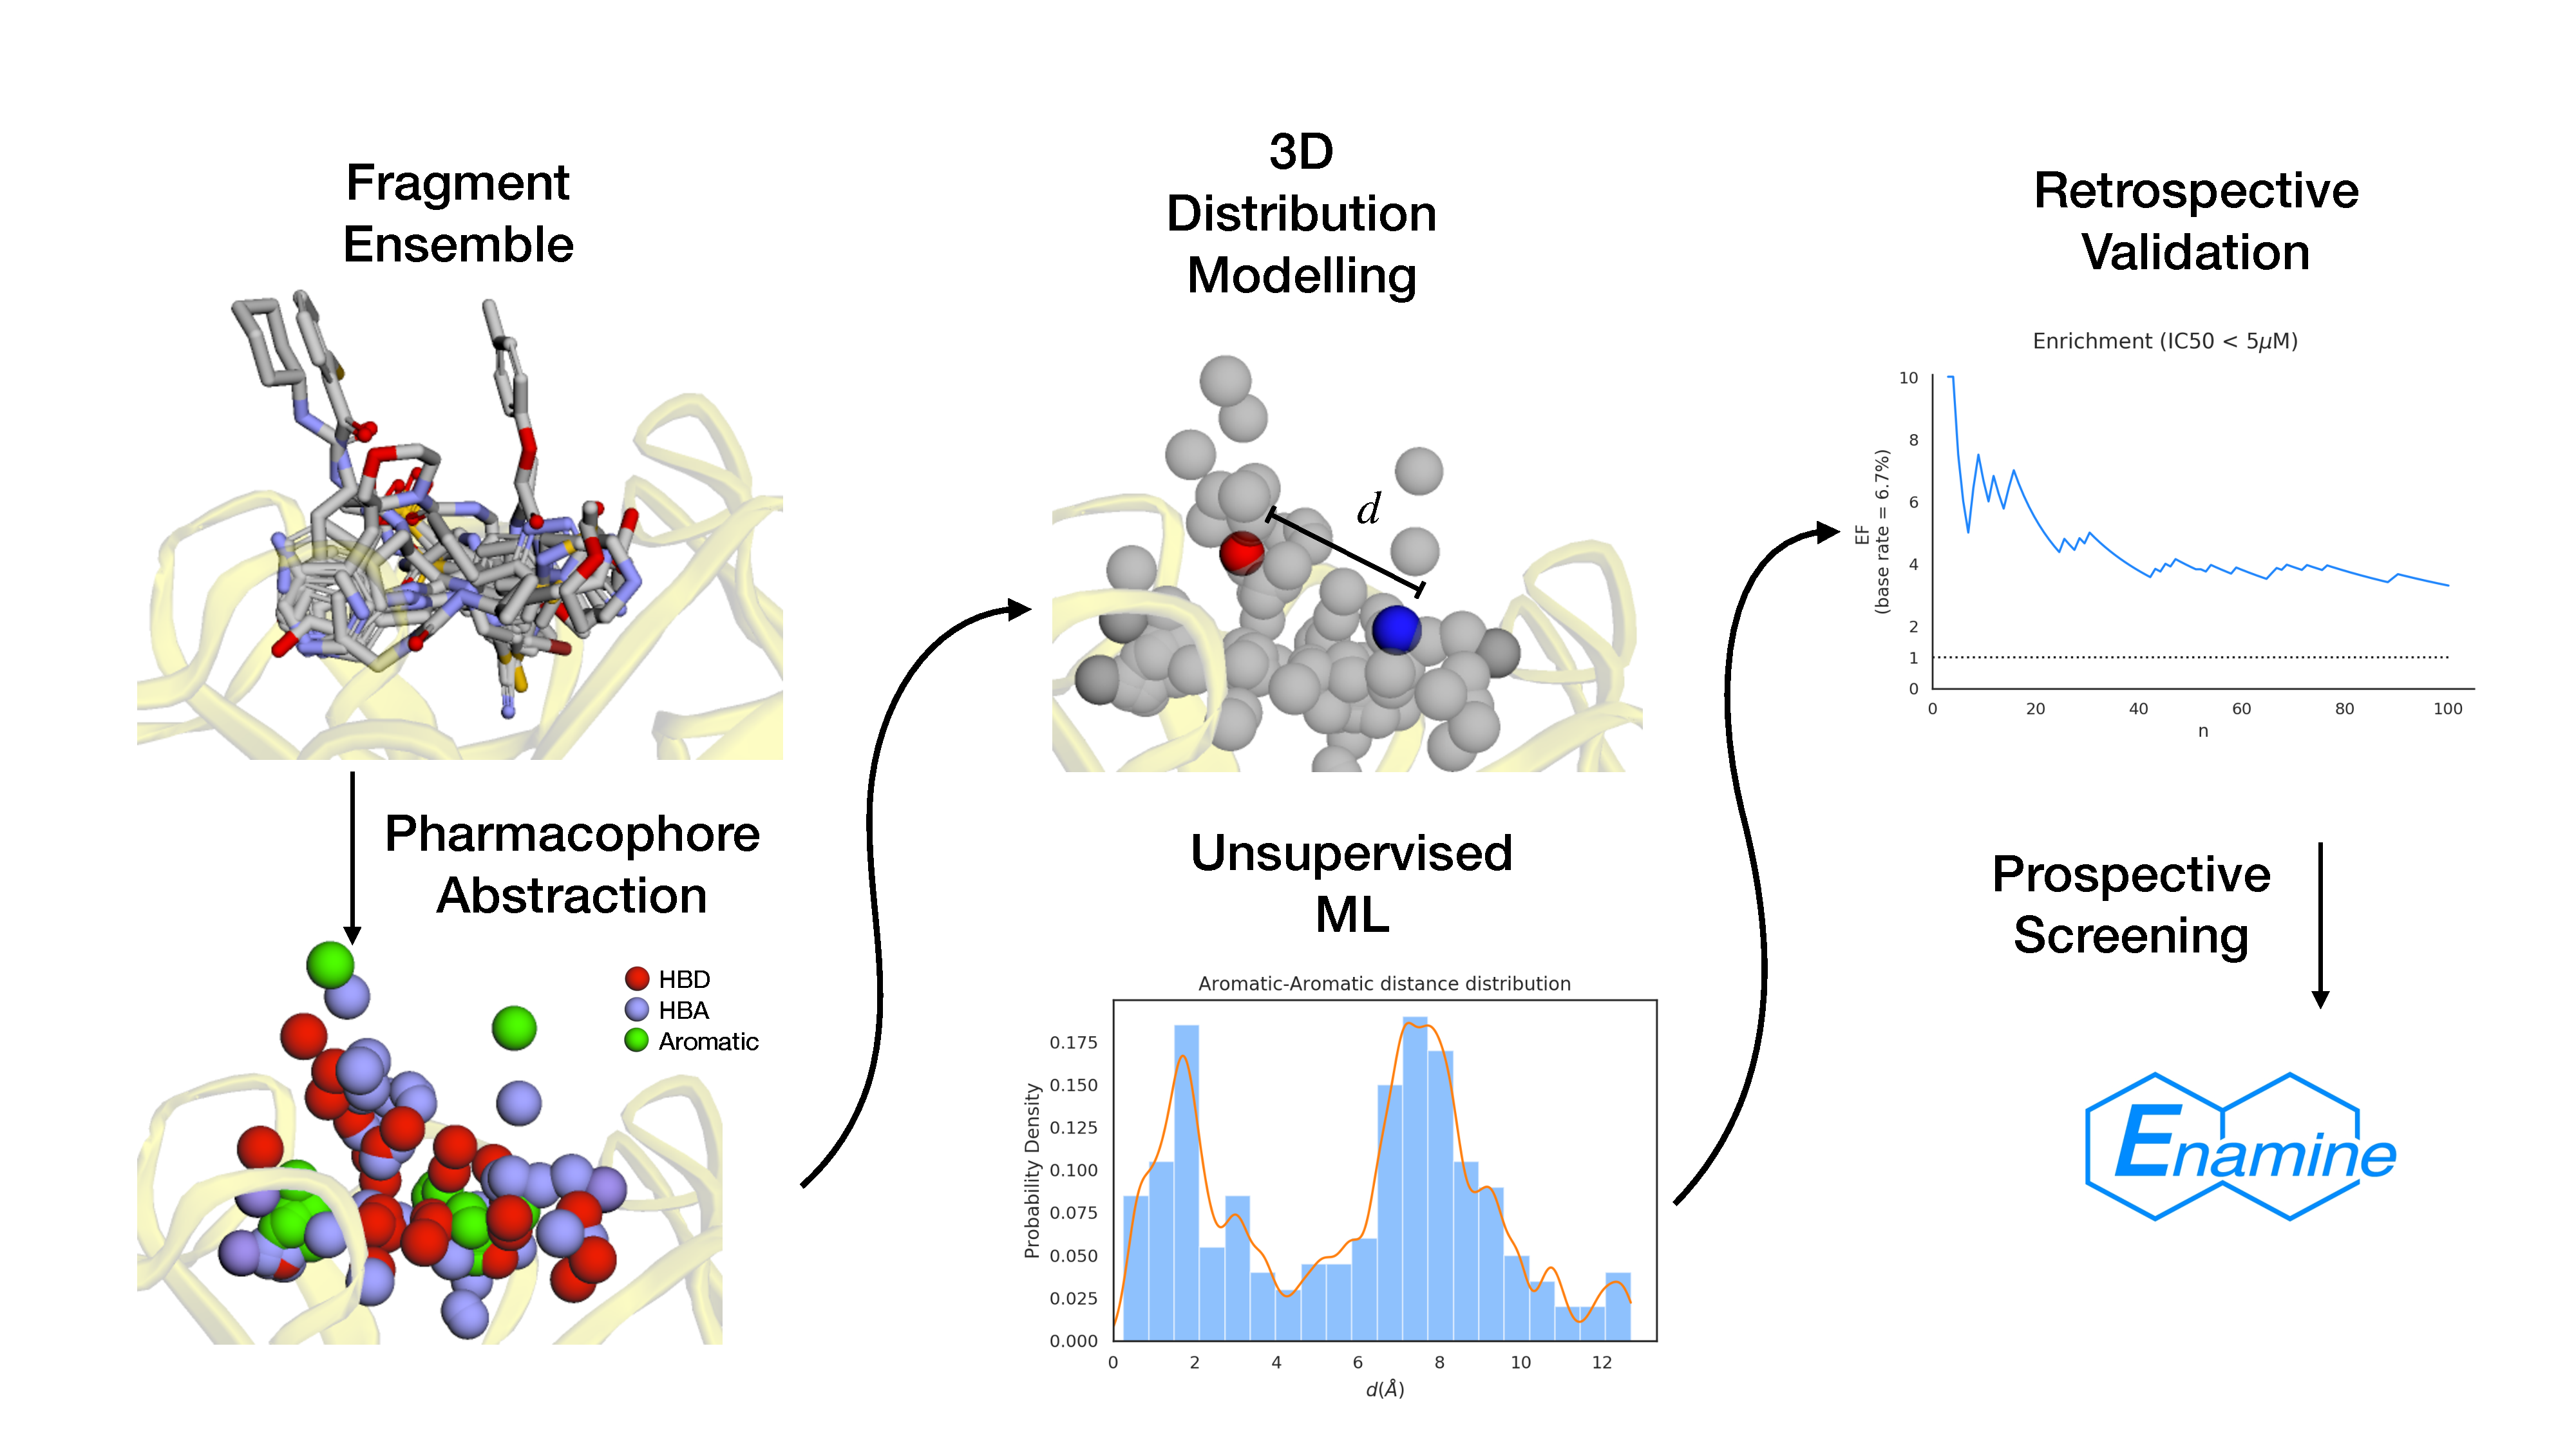
\includegraphics[
  height=3.5cm,
  keepaspectratio,
]{figs/frag_fig1.pdf}
\end{center}
\end{tocentry}

\begin{abstract}
In this work, we describe an end-to-end hit detection approach that bridges the the paradigms of both fragment-based drug design and virtual screening. Our method, named FRESCO, utilises unsupervised learning to learn pharmacophore distributions directly from experimental 3D fragment-protein structures. The trained model evaluates whether or not a particular compound possesses pharmacophores matching the distribution exhibited by the bound fragments, replicating the intuition of a medicinal chemist deducing spatial correlations between pharmacophores from different fragments. Our approach is computationally validated with a retrospective study on SARS-CoV-2 main protease (Mpro) ligands using data from COVID Moonshot \cite{Moonshot2022}, showing high enrichment. Then, we conduct an experimental search for novel hits for Mpro and the Mac1 domain of SARS-CoV-2 non-structural protein 3 (nsp3) by scoring a library of 1.4 billion purchasable compounds from EnamineREAL, resulting in 1 (novel?) hit for MPro and 2 (novel?) hits for Mac-1. (Scaffold exploration of the detected hits hopefully lead to novel potent ligands!) Our results are the first experimentally validated demonstration of hit detection via a fully computational workflow starting directly from an experimental fragment screen.
\end{abstract}

%%%%%%%%%%%%%%%%%%%%%%%%%%%%%%%%%%%%%%%%%%%%%%%%%%%%%%%%%%%%%%%%%%%%%
%% Start the main part of the manuscript here.
%%%%%%%%%%%%%%%%%%%%%%%%%%%%%%%%%%%%%%%%%%%%%%%%%%%%%%%%%%%%%%%%%%%%%
\section{Introduction}

TODO - shorten introduction, put some of it in discussion?

Developing a new drug from original idea to the launch of a finished product is a complex process which can take 12–15 years and cost in excess of \$1 billion \cite{Hughes2011Principles}. A key step in the early stages of the drug discovery process following the identification of a biological target is hit detection. Broadly speaking, a `hit' is a compound that interacts with the identified target sufficiently strong enough to act as a starting point for optimisation of the compound structure towards a candidate drug. 

Approaches towards hit detection generally involve the screening of libraries of compounds. For example, in high throughput screening (HTS) often hundreds of thousands of chemical compounds are synthesised and tested, requiring substantial resources as well as complex logistics. While experimental techniques such as DNA-Encoded libraries are being developed to increase the efficiency of large-scale compound screening \cite{GirondaMartinez2021DNALibrary}, there has been a growing push towards conducting hit detection computationally instead to decrease the cost and accelerate this step of the drug discovery process \cite{?}. 

In this approach, known as virtual screening, a computational scoring function is used to estimate the potency of a compound. After computing the scores for all of the compounds in a library, only those ranked highly by the scoring function are chosen for synthesis and experimental validation. Currently the predominant scoring function used to conduct a virtual screen is molecular docking. In molecular docking, the 3D conformation of a ligand and the target are explicitly modelled and a physics-based simulation of the binding process is conducted, with the calculated energy of the bound ligand as the score. Although this approach has yielded success \cite{Lyu2019UltraLargeDocking,Alon2021SigmaTwo}, correctly performing molecular docking is non-trivial and the deficiencies of molecular docking for bioactivity prediction are well-documented \cite{Llanos2021StrengthsAndWeaknesses, Macip2022HasteMakesWaste}.


\begin{figure}
    \centering
    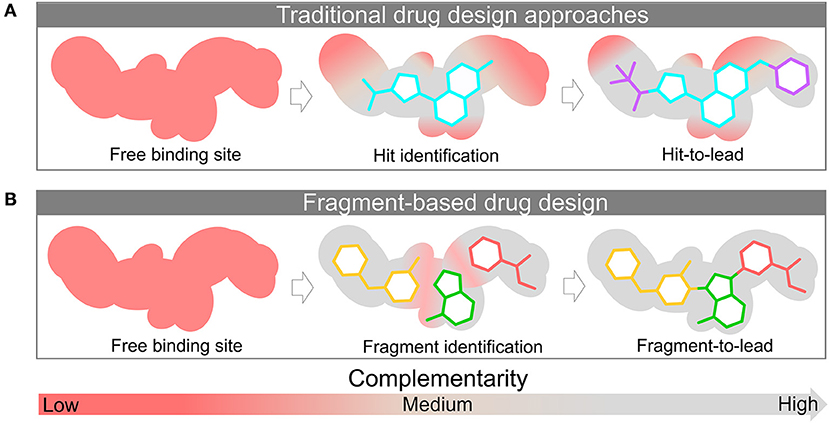
\includegraphics[width=\linewidth]{figs/fbdd_vs_trad.jpg}
    \caption{An illustration comparing fragment-based drug discovery to traditional approaches.}
    \label{fig:fbdd}
\end{figure}

An alternative to these methodologies is fragment-based drug discovery (FBDD). In this approach, a library of very low molecular weight compounds (`fragments' typically less than 18 nonhydrogen atoms \cite{David2017FBLD}) are screened at high concentrations alongside the generation of bound fragment-protein structures via X-ray crystallography or cryo-EM. By obtaining these experimental structures and examining the binding interactions between individual fragments with protein residues, fragments can be used as building blocks for larger molecules by linking or merging together disparate fragments in order to increase potency. Conceptually, FBDD is based on a coarse-graining of fragments to specific moieties or groups that are associated with interactions to the target, with the goal of maintaining and optimising these interactions in larger molecules.

 Although there exist some computational approaches for supporting FBDD, for example hot spot analysis and pocket druggability prediction \cite{deSouza2020InSilicoFBDD}, at present the main procedure of selecting which fragments to merge and how to do so remains largely intuition-based and human-driven. (and fraught to error? citation needed \cite{?})

In this work, we describe an end-to-end hit detection approach that bridges the the paradigms of both fragment-based drug design and virtual screening. Our method, named FRESCO, utilises unsupervised machine learning to learn pharmacophore distributions directly from experimental 3D fragment-protein structures. The trained model acts as a scoring function that can be used to perform virtual screening, evaluating whether or not a particular compound possesses pharmacophores matching the distribution exhibited by the bound fragments. 

This methodology aims to replicate the intuition of a medicinal chemist preforming fragment-based drug discovery, abstracting fragments to pharmacophores and deducing spatial correlations between pharmacophores from different fragments. As a matter of fact, we go beyond the typical strategem of growing one individual fragment independently of the others, or merging two particular fragments - by training our model on all of the fragment-protein structures we leverage information from all existing fragments, ensuring no pharmacophore correlations are overlooked in the hit detection process.

We first computationally validate our approach with a retrospective study on bioactivity prediction for SARS-CoV-2 main protease (Mpro) ligands using data from COVID Moonshot \cite{Moonshot2022}, showing high enrichment. Then, we conduct an experimental search for novel hits for Mpro and the Mac1 domain of SARS-CoV-2 non-structural protein 3 (nsp3) by performing a virtual screen with FRESCO on a library of 1.4 billion purchasable compounds from EnamineREAL. This resulted in 1 (novel?) hit for MPro and 2 (novel?) hits for Mac-1, with crystallographic poses for the Mac-1 hits. Follow-up compounds for performing scaffold exploration of the detected hits were synthesised and assayed demonstrating credible structure-activity relationships, confirming that the detected hits were genuine.

Our method is unique not only in its philosophy, but also its use of unsupervised learning in the form of kernel density estimation. Although there has been a rapid growth in machine learning methods applied to drug discovery in recent years particularly in QSAR/molecular property prediction, the vast majority of them are supervised learning techniques requiring not merely the existence of experimental assay data, but its existence in sufficient quantity and quality to train a useful model. The nature of the problem of hit detection in early-stage drug discovery is one where such data in nonexistent, which underlies the necessity of having methods for directly performing hit detection from fragment screen data. 

The only comparable methods that the authors are aware of is recent work in using deep generative models for proposing merges between two fragments (DeLinker \cite{Imrie2020DeLinker}, SyntaLinker \cite{Yang2020SyntaLinker}, and Develop \cite{Imrie2021Develop}). These approaches differ for ours in several ways: Firstly, these models all require human intervention from an expert in choosing which fragments to merge, or what pharmacophoric constraints need to obeyed, whereas our model is fully end-to-end. Secondly, these methods utilise neural network-based generative models which are very sensitive to training hyperparameter choice in general (citation about mode collapse \cite{?}), and for molecular generation in particular known to propose invalid and/or unsynthesizable molecules \cite{Gao2020Synthesizability}. In contrast, our method relies on kernel density estimation which is simple, robust and free from hyperparametear tuning, and we we explicitly only screen purchasable, easily-synthesised molecules. Lastly, the proposed models have only been studied computationally and lack validation in the real world.

Our results are the first experimentally validated demonstration of hit detection via a fully computational workflow starting directly from an experimental fragment screen. This work opens the door for bridging fragment-based drug discovery with virtual screening.

\section{Results}


\subsection{Computational Retrospective Study}

To validate that our hypothesised methodology has merit, a computational study was conducted on the SARS-CoV-2 main protease (Mpro). The COVID Moonshot campaign \cite{Moonshot2022} was established as an open science effort towards developing a patent-free antiviral drug for the SARS-CoV-2, specifically targeting the inhibition of Mpro as that would prevent the virus from further replication. Throughout the campaign, activity data consisting of the structures of molecules that were synthesised and assayed was continually released. As a proof-of-concept, the model predictions for the assayed molecules are compared against the measured activity and analysed.

Firstly, the FRESCO model was fit on publicly reported crystallographic structures of non-covalent fragments bound to the SARS-CoV-2 Mpro protein \cite{Douangamath2020XChem}. Next, conformer coordinates for Moonshot compounds reported before March 22nd 2021 were obtained from parallel work within the Moonshot consortium performing docking studies on Mpro (TODO - citation/explanation?). Pharmacophore features were generated from these conformers and the molecules were scored using the model. The enrichment factor for picking compounds above an IC50 of 10\uM is computed as we are most interested in the ability of this model to sample potent compounds. We also compute the enrichment from ranking the compounds with the Chemgauss4 scoring function.

\begin{figure}
    \centering
    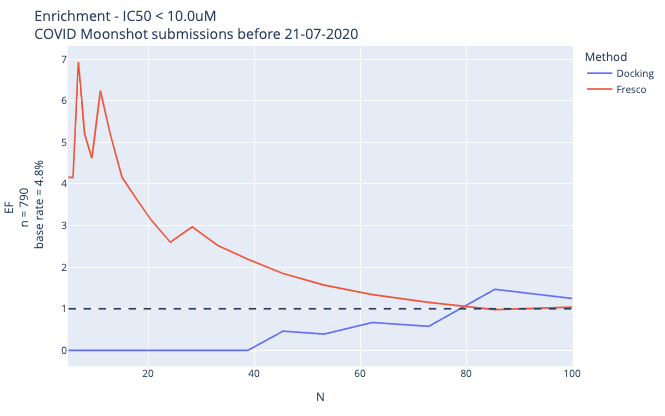
\includegraphics[width=\textwidth]{figs/enrichment_vs_docking.png}
    \caption{FRESCO is able to detect potent compounds purely based on unsupervised learning. High enrichment relative to docking is achieved when performing a retrospective study on activity data COVID Moonshot.}
    \label{fig:moonshot_enrichment_vs_docking}
\end{figure}

The results are shown in Fig. \ref{fig:moonshot_enrichment_vs_docking} illustrating high enrichment, validating the hypothesis that it is possible to correlate bioactivity with unsupervised learning of fragment pharmacophore distributions. The date 21st July 2021 marks when additional experimental data was released and the direction of the COVID Moonshot campaign shifted from hit detection to optimisation of existing lead compounds \cite{Moonshot2021DataRelease}. The optimisation process relies on the improvement of energetic interactions between the ligand and residues in the active site, likely growing beyond the volume covered by the initial fragment hits and so cannot in principle be captured by FRESCO. This is consistent with the observed decrease in enrichment relative to docking when using data from latter stages of Moonshot where more of the submitted compounds are designed for reaching nanomolar affinity. This shows the value in using FRESCO for hit detection in the early stages of a drug discovery campaign.

TODO - Which enrichment curves to show? Put some in the SI? Should I include ZINC graph?

\subsection{Experimental Prospective Study}
After confirming the merit of this approach via a retrospective computational study, a prospective experimental search for novel hits was performed to demonstrate the capability of this methodology. We study two targets: the main protease (Mpro) of SARS-CoV-2 and the Mac1 domain of SARS-CoV-2 non-structural protein 3 (nsp3). 

For both targets we followed the same workflow to discover novel hits. We first fit FRESCO models on experimental fragment-protein crystal complexes, and used the models to screen the VirtualFlow \cite{Gorgulla2020VirtualFlow} library of commercially available compounds. The top predicted compounds were filtered by their physical properties and were clustered by structural similarity. The centroids of the 50 most populous clusters were selected as hit candidates and ordered for synthesis and testing. Details on the methodology can be found in Sec. \ref{sec:methods}.

\subsubsection{Mpro}
For Mpro, 38 compounds were successfully synthesised and assayed. One of the compounds, WIL-UNI-d4749f31-37, was recorded with an IC50 of 25.8\uM measured via fluorescence assay while the remaining compounds were found to be inactive. To confirm that the compound activity was not a false positive (eg measured potency due to assay interference) and that genuine ligand-protein interactions existed, a follow-up series of 8 compounds (ALP-UNI-ed5cdfd2) consisting of structural perturbations to the molecular scaffold was also synthesised and assayed. All 8 compounds exhibited inhibition at high concentrations and one compound (ALP-UNI-ed5cdfd2-1) had a lower IC50 of 19.4\uM, demonstrating a genuine structure–activity relationship SAR for this hit compound.

Mpro order 1st batch = WIL-UNI-d4749f31, order 2nd batch = WIL-UNI-2a57d06c (no actives). 

\begin{figure}
    \centering
    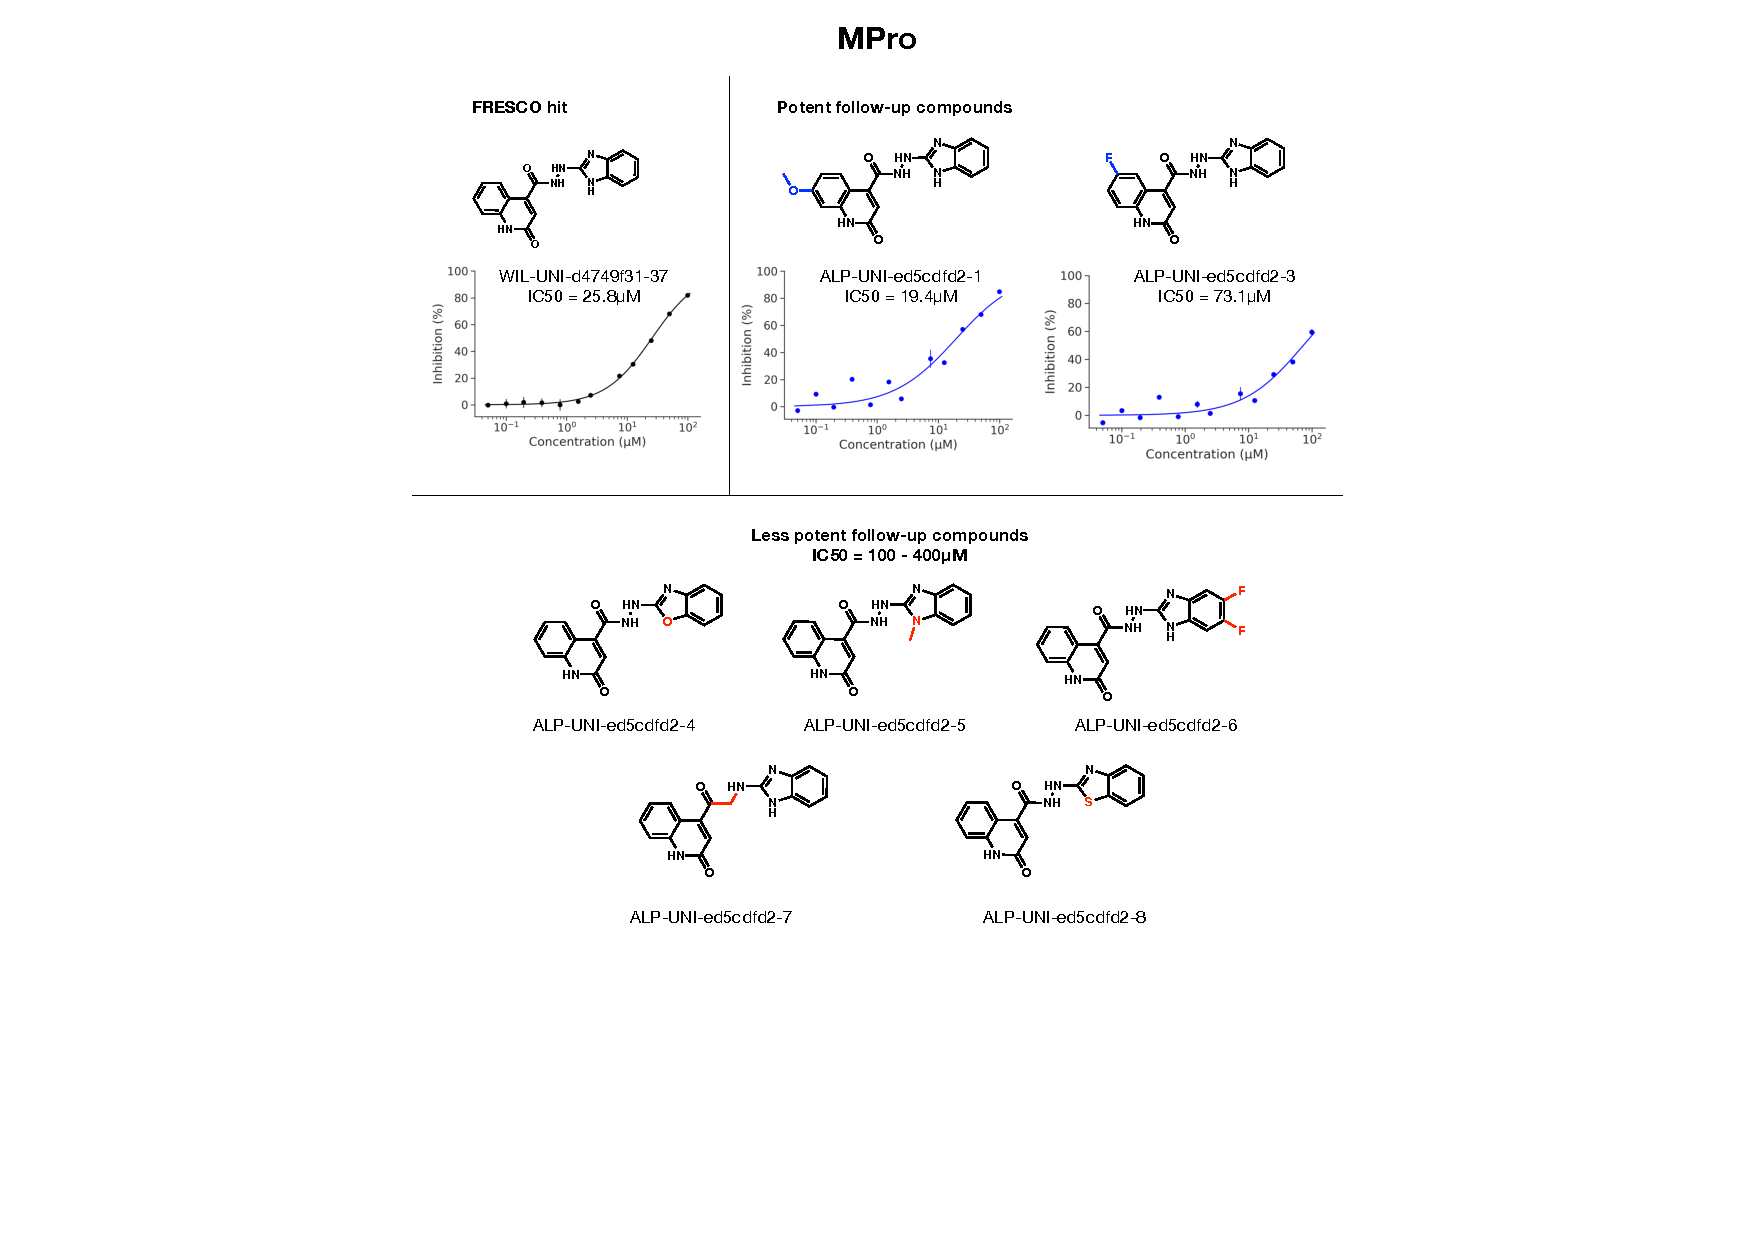
\includegraphics[width=\linewidth]{figs/mpro_hit_IC50.png}
    \caption{Dose-Response curve for WIL-UNI-d4749f31-37 and follow-up compounds demonstrating SAR relationship.}
    \label{fig:mpro_hit}
\end{figure}

\subsubsection{Mac-1}
For Mac-1, 52 compounds were successfully synthesised and assayed. Two of the compounds show non-negligible activity at high concentration - at 250\uM, compound Z5551425673 (as a racemic mixture) has an inhibition of 30.1\% , while compound Z1102995175 has 24.8\%. In addition, crystallographic structures of Z5551425673 (modelled as the S-stereoisomer) bound to the active site was also found alongside that of 3 other compounds (Z2890189003, Z2890182452, Z1423250928), confirming that Z5551425673 is a true hit.

As with Mpro, a follow-up series of compounds were designed to perturb the chemical structure of Z5551425673 in order to confirm the existence of SAR for this compound against Mac-1. 26 compounds were ordered and ... TODO.

\begin{figure}
    \centering
    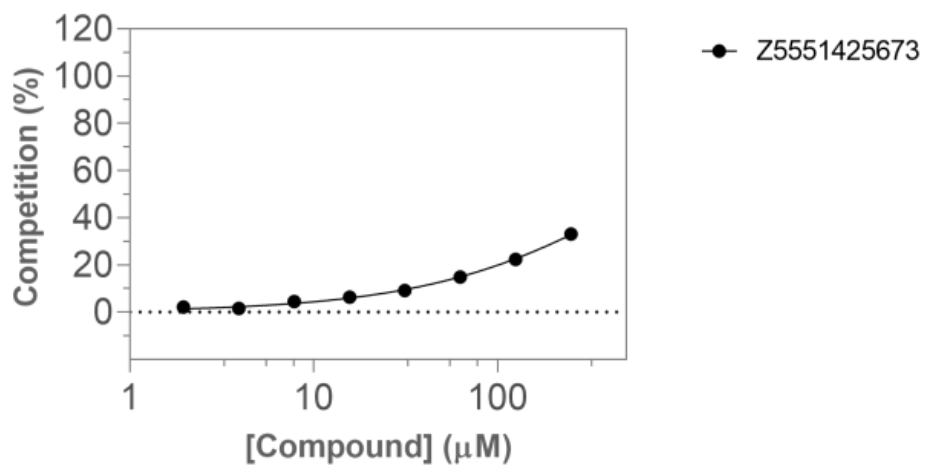
\includegraphics[width=\linewidth]{figs/mac1_hit_IC50.png}
    \caption{Dose-Response curve for Z5551425673 and follow-up compounds demonstrating SAR relationship. Also showing crystal structure TODO.}
    \label{fig:mac1_hit}
\end{figure}

TODO - table and structures in SI

\section{Discussion}

TODO - improvements that could be made? Future extensions? Transfer learning between targets? Docked fragments? Ensemble dock scores with FRESCO scores?

\section{Conclusion}

\section{Methods} \label{sec:methods}
\subsection{Datasets}

The crystal structures were downloaded from \href{https://fragalysis.diamond.ac.uk/viewer/react/landing}{\texttt{Fragalysis}}. For Mpro, non-covalent fragments from the XChem fragment screen \cite{Douangamath2020XChem} were used while for Mac-1 both XChem and UCSF fragment data were used.

The Moonshot activity data for the retrospective study was accessed in Mar 22nd 2021. The IC50 values in that dataset, as well as in the prospective study on Mpro were measured from a fluorescence based enzyme activity assay.

For Virtual Screening, we utilize a published dataset of more than 1.4 billion commercially available molecules from EnamineREAL \& ZINC15 in a ready-to-dock format \cite{Gorgulla2020VirtualFlow}.

\subsection{Model Construction}
The model used in this work takes as input the 3D pharmacophore distribution of a candidate molecule, and evaluates the log-probability that the distribution matches that of the fragment screen on the target site.

The 3D pharmacophore distribution of a molecule is obtained by extracting pharmacophores from the molecular SMILES and their corresponding conformer coordinates, and then evaluating the pairwise distance matrix between all possible pharmacophore pairs (eg Donor-Donor \& Aromatic-Acceptor). SMARTS pattern matching following default pharmacophore definitions in \href{https://www.rdkit.org/docs/index.html}{\texttt{RDKit}} were used to extract pharmacophores from the fragment SMILES. The pharmacophores considered are hydrogen bond donors, hydrogen bond acceptors, and aromatic rings. The coordinates of each pharmacophore are defined as the average over the atoms in the pharmacophore (eg the position of an aromatic pharmacophore from a benzene ring would be the mean of the coordinates of the 6 carbon atoms in the ring). 

For some fragments, multiple crystallographic poses are recorded. To account for this, we weigh the contribution of each fragment structure to the overall fragment pharmacophore distribution by $\frac{1}{n}$ where $n$ is the number of conformations recorded for each conformer. In addition, we exclude the counting of correlations between pharmacophores from the same fragment - only correlations between different fragments are measured. This is to avoid spurious intra-fragment correlations that have nothing to do with binding to the binding site - strong correlations in pharmacophore distribution between multiple independent fragments are indicative of useful binding interactions and these are what we hope to capture with this methodology.

The bandwidth for KDE fitting was chosen for each system using the Improved Sheather-Jones algorithm \cite{Botev2010ISJ} (implemented in \href{https://kdepy.readthedocs.io/en/latest/index.html}{\texttt{KDEpy}}). KDEs of the systems are then constructed using the chosen bandwidths with \href{https://scikit-learn.org/stable/}{\texttt{scikit-learn}} for technical ease of use in evaluating probabilities. The \texttt{scikit-learn} implementation relies on a relatively slow tree-based algorithm that searches over the training datapoints - to increase the efficiency of virtual screening, computationally fast approximations of the KDEs are made using the \texttt{scipy} \href{https://docs.scipy.org/doc/scipy/reference/generated/scipy.interpolate.interp1d.html#scipy.interpolate.interp1d}{\texttt{interp1d}} function. Comparisons of the KDE bandwidth can be found in supplementary information.

Virtual screening of molecular libraries is done by evaluating the probability of the pharmacophore distribution of each molecule using the KDEs. For each pharmacophore combination, the mean log-probability of the distribution is calculated. The overall score for the molecule is returned as the mean log-probability over all of the pharmacophore combinations.

TODO - description of runtime? Emphasise no GPUs needed?

\subsection{Compound Selection}
After conducting a virtual screen, the top-500k predictions were selected and filtered to remove undesirable properties. A series of successive filtering steps were performed: first, only molecules with physical properties in well-understood ``lead-like'' chemical space \cite{ChemSpace} were kept. Secondly, the sum of the number of hydrogen bond donors and hydrogen bond acceptors were constrained to an upper limit of 8 as we noticed that the model tended to pick ``messy'' molecules. Then, we remove molecules that match known filters for pan-assay interference compounds (PAINS) \cite{Baell2010Pains} as well as filters for covalent substructures (eg furan, thiophene, nitro groups). Duplicate tautomers for each molecule are also removed. Finally, for ease of synthetic accessibility, we only consider molecules with less than two chiral centers.

The top-50k molecules remaining from the filtering were then clustered via Butina Clustering \cite{Butina1999Clustering} with a Tanimoto distance threshold of 0.2. This resulted in 24748 and 22358 clusters for Mpro and Mac-1, respectively. For both targets the centroids of the 50 most populous clusters (or the closest purchasable analogue if it wasn't available) were chosen as the candidate compounds. These compounds were ordered for synthesis from Enamine which resulted in 38 and 52 successfully made molecules for Mpro and Mac-1, respectively.

TODO - Confirm made/assayed molecule numbers.

\section{Author Contributions}
WM and AAL designed the study. WM and AAL devised the predictive model and WM implemented it. WM and AAL wrote the original draft, all authors commented on it.

\begin{acknowledgement}

WM acknowledges the support of the Gates Cambridge Trust. AAL acknowledges the Winton Programme for the Physics of Sustainability.

\end{acknowledgement}

\begin{suppinfo}

All code used for this work can be found in the GitHub repo \url{https://github.com/wjm41/frag-pcore-screen}. Supplementary figures and tables can be found in an accompanying file.

\end{suppinfo}

\bibliography{refs}

\end{document}